\section{Prerequisites}

Prior to implementing the required LS\footnote{Least Square} and RLS\footnote{Recursive Least Square} algorithms, we need to have an understanding of the given transfer function and its corresponding system. In this section we evaluate the step and frequency responses of the transfer function and in doing so, gather much needed information on timing and frequency charactristics of the given system. 

Given  \autoref{eq:preTransferFunction}, we calculate the settling time of the step response to properly discretize our system. We simplify the parameters of the  \autoref{eq:preTransferFunction} and make the denominator monic as shown in  \autoref{eq:preTransferFunction2}. 

\begin{equation}
	G(s) = \frac{2(0.6s + 1)^2}{(3s + 1)(2s + 1)(s + 1)}
	\label{eq:preTransferFunction}
\end{equation}

\begin{equation}
	G(s) = \frac{0.72s^2 + 2.4s + 2}{6s^3 + 11s^2 + 6s + 1}
	\label{eq:preTransferFunction2}
\end{equation}

%%%%%%%%%%%%%%%%%%%%%%%%%%%%%%%%%%%

The Matlab codes provided in preceeding section are residing at \hspace{-1ex}\lstinline| assignment1/part1/1_0/LS1_0.m| file. The equavilant Matlab code of the transfer function is displayed in  \autoref{code:preSettelingTime}. While irrelevant code segments have been removed, the original line numbers are retained to ensure consistency with the associated MATLAB files. The calculated setteling time is $14.72$ seconds and the sample time is $0.3$ of a second. The step response plot is shown in  \autoref{fig:preStepResponse}.

\begin{code}
	\begin{matlabcode}{firstnumber = 4}
		%% Evaluate transfer function
		s = tf('s');
		G = (0.72*s^2 + 2.4*s + 2) / (6*s^3 + 11*s^2 + 6*s + 1);
		
		%% Plot step response
		figure;stepplot(G);grid on;fontsize( 24 ,"points");
		
		%% Get settling time of step response
		s = stepinfo(G);
		
		%% Calculate the time interval for sampling
		sampleTimeIntervals = s.SettlingTime/50;
		fprintf("Settling time:%f\nSample time:%.2fs\n", ...
		s.SettlingTime,round(sampleTimeIntervals,1));
	\end{matlabcode}
	\captionof{listing}{Setteling time calculation in Matlab}
	\label{code:preSettelingTime}
\end{code}

\begin{figure}
	\centering
	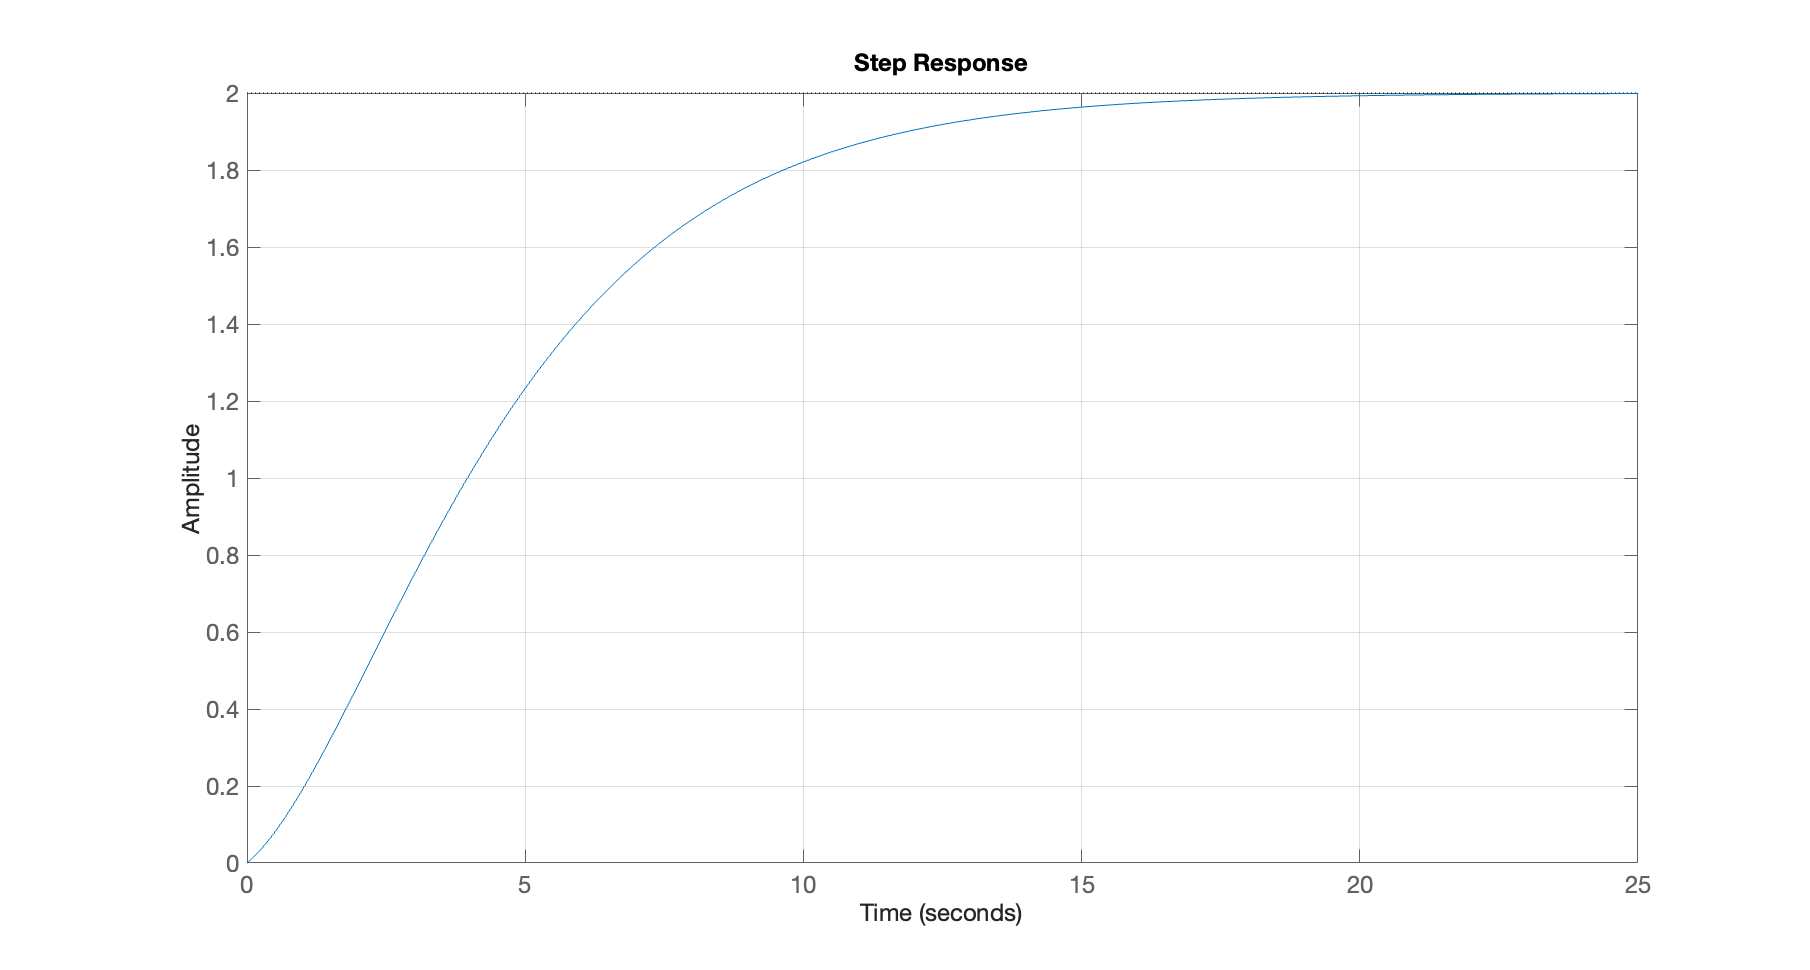
\includegraphics[width=\textwidth]{images/preStepResponse.png}
	\caption{Step response}
	\label{fig:preStepResponse}
\end{figure}

%%%%%%%%%%%%%%%%%%%%%%%%%%%%%%%%%%%

We then evaluated the frequency response of \autoref{eq:preTransferFunction2} using the MATLAB code in \autoref{code:preFrequencyResponse}, which generates the Bode plot and calculates the maximum suitable frequency. The calculations revealed that the input sine wave frequency must be less than 0.1 $\frac{rad}{s}$. The Bode diagram is presented in \autoref{fig:preFrequencyResponse}.

\begin{code}
	\begin{matlabcode}{firstnumber = 20}
		%% Bode plot of G
		figure;bodeplot(G);grid on;fontsize( 24 ,"points");
		
		%% Calculate the frequency response
		w = logspace(-1, 2, 1000); % Frequency vector
		[mag, phase] = bode(G, w); % Or use freqs(sys,w)
		
		%% Find the 3dB frequency
		w = logspace(-1, 2, 1000);
		[mag, phase] = freqresp(G, w);
		[max_mag, max_index] = max(abs(mag));
		max_freq = w(max_index);
		fprintf('Maximum magnitude: %.4f\n', max_mag);
		fprintf(['Frequency for sine input needs to be less than:''%.2f rad/s\n'], max_freq);
	\end{matlabcode}
	\captionof{listing}{Frequency response in Matlab}
	\label{code:preFrequencyResponse}
\end{code}

\begin{figure}
	\centering
	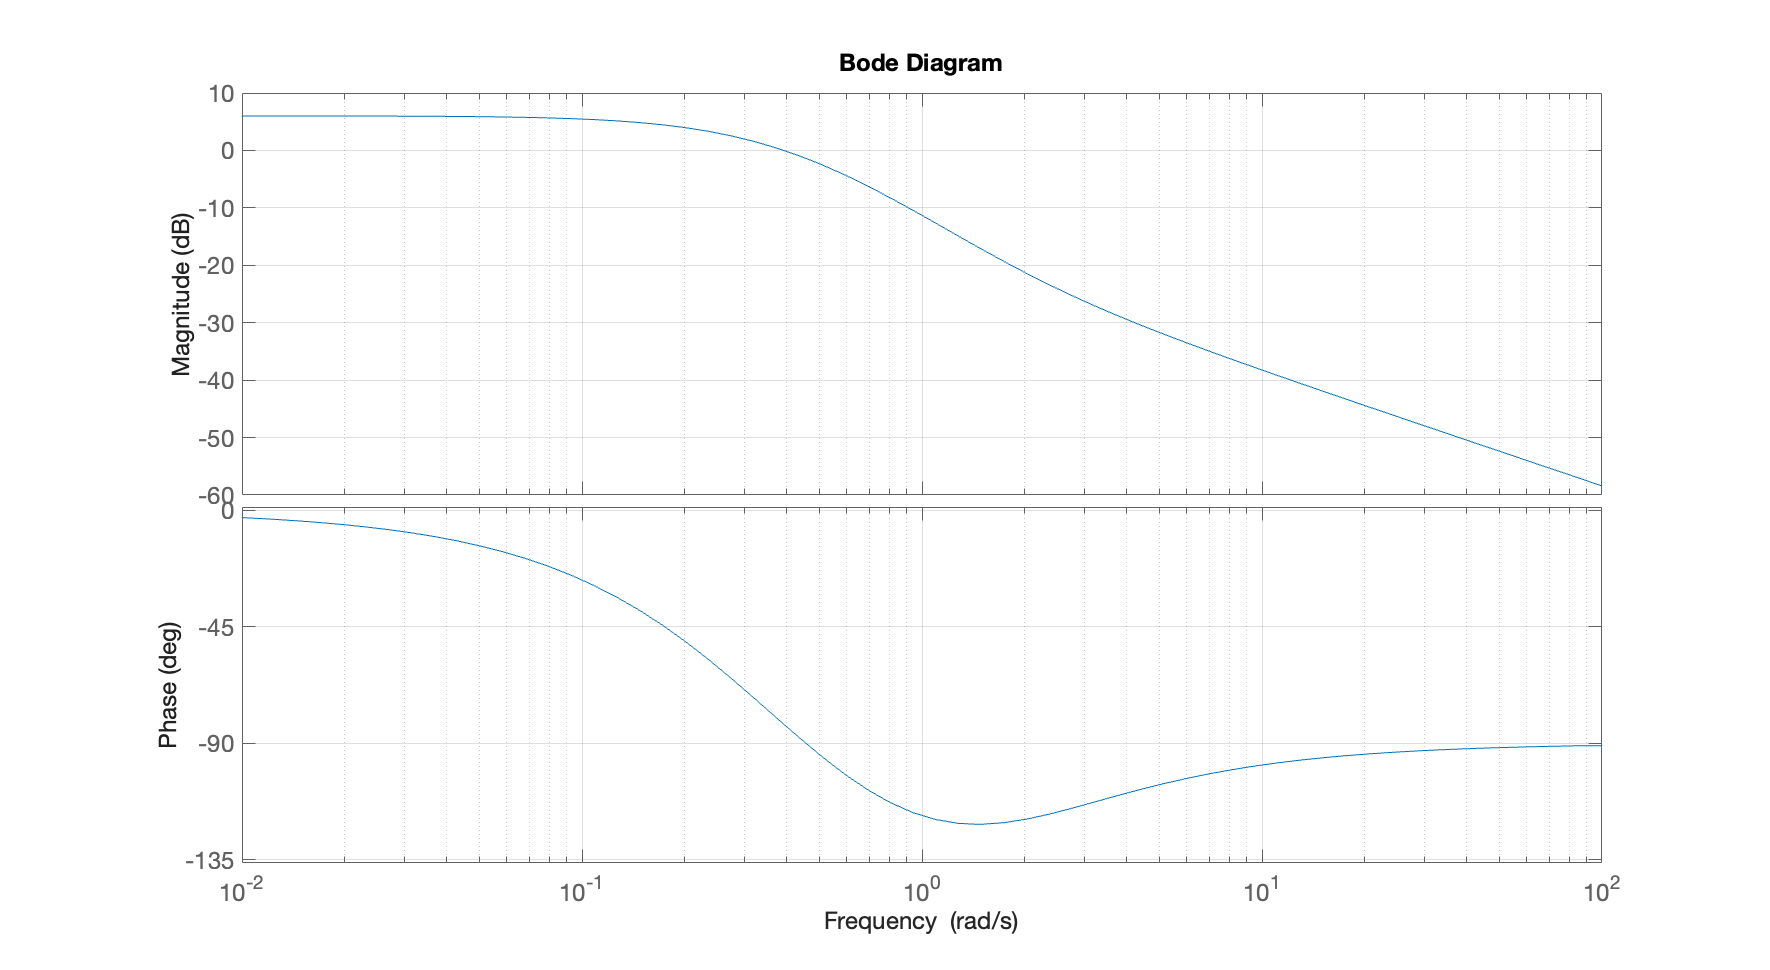
\includegraphics[width=\textwidth]{images/preBodeDiagram.png}
	\caption{Frequency response}
	\label{fig:preFrequencyResponse}
\end{figure}

%%%%%%%%%%%%%%%%%%%%%%%%%%%%%%%%%%%

When a $2\sin(0.1t)$ input was applied to the system, the output exhibited a minimum value of $-3.75$ and a maximum of $3.76$, as shown in \autoref{fig:preSineResponse}. This resulted in a peak-to-peak value of $7.51$. The MATLAB code used for this evaluation is provided in \autoref{code:preSineResponse}, and the input and output sine waves are visualized in \autoref{fig:preSineResponse}.

\begin{code}
	\begin{matlabcode}{firstnumber = 36}
		%% Define the sine wave input
		t = 0:0.01:100;
		u = 2*sin(0.1*t);
		
		[y,t] = lsim(G, u, t);
		
		figure;subplot(2,1,1);plot(t, u);fontsize( 24 ,"points");
		title('Input Signal (2*Sine(0.1*t) Wave)');
		xlabel('Time (s)');ylabel('Amplitude');
		subplot(2,1,2);plot(t, y);fontsize( 24 ,"points");
		title('Output Signal');xlabel('Time (s)');ylabel('Amplitude');
		fprintf(['The sine rsponse for 2*sine(0.1*x) has min: %0.2f max: %0.2f peak2peak: %0.2f\n'],min(y),max(y),peak2peak(y));
	\end{matlabcode}
	\captionof{listing}{Sine response in Matlab}
	\label{code:preSineResponse}
\end{code}

We will take advantage of frequency response and given sine reponse information when adding noise to the output of the system. By knowing the amplitude of the output, we can easily determine the $0.1$ or $10\%$ of that ampilitude and generate the required noise accordingly. 

\begin{figure}
	\centering
	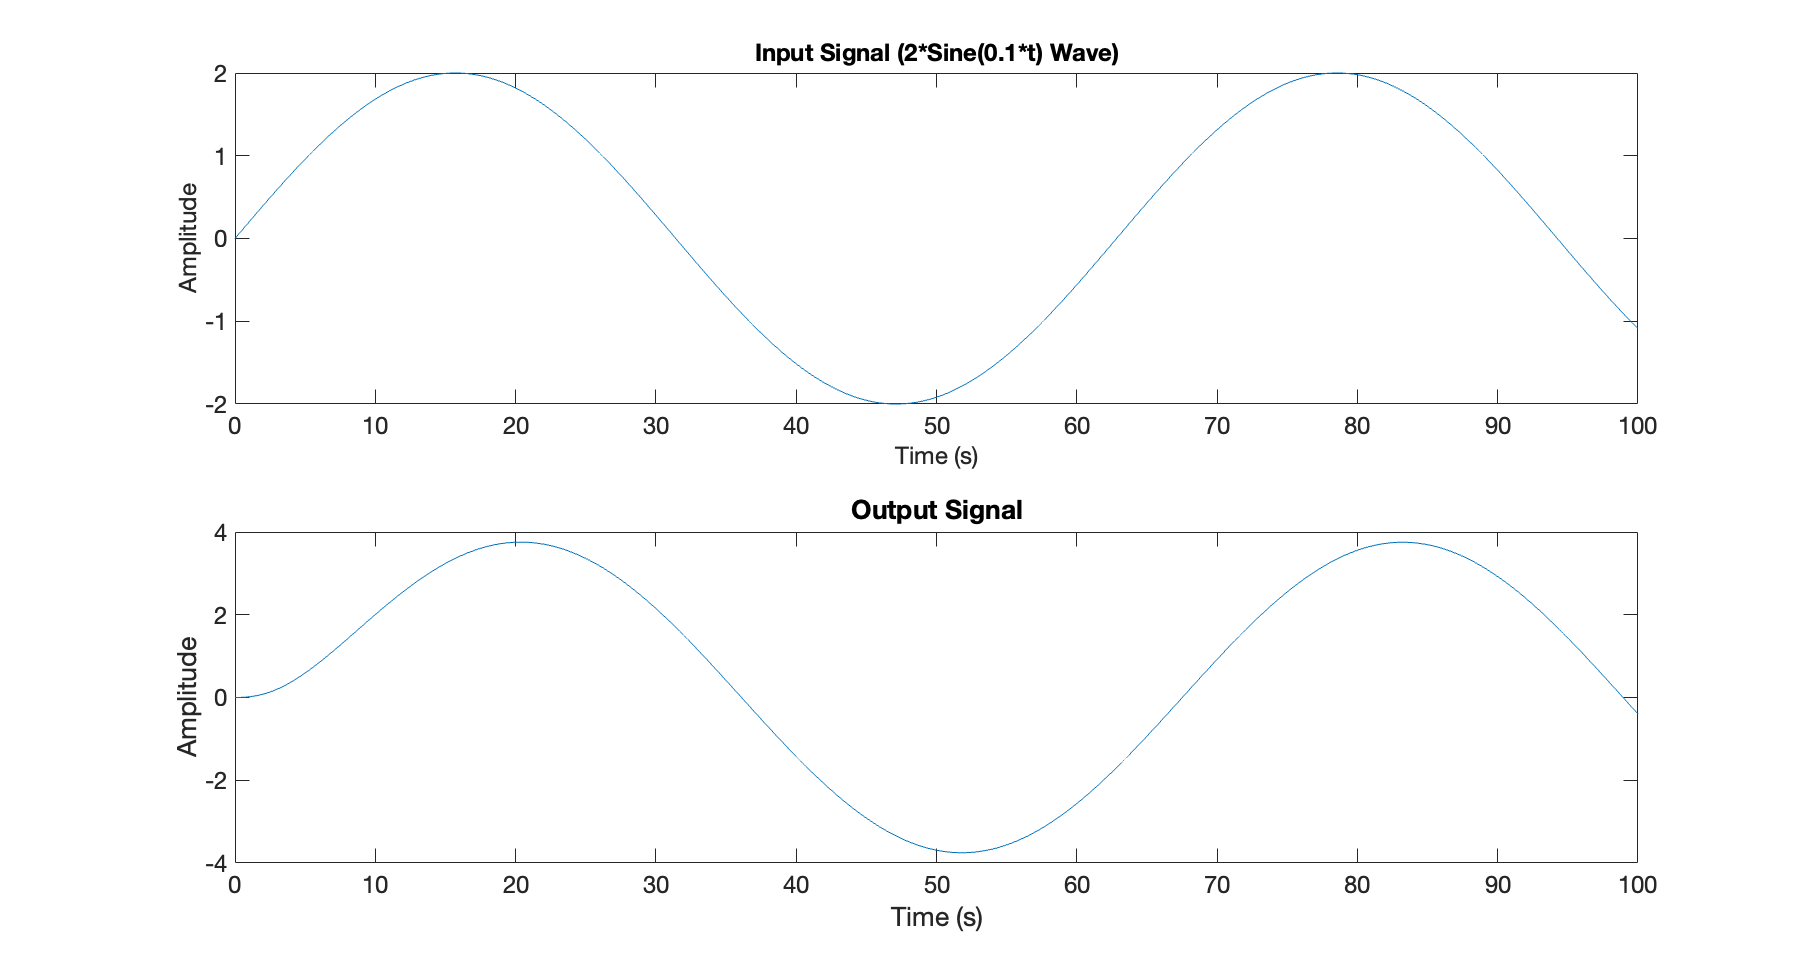
\includegraphics[width=\textwidth]{images/preSineResponse.png}
	\caption{Sine response}
	\label{fig:preSineResponse}
\end{figure}
